% Q16：按原图线型重绘斜三棱柱及辅助线；空间位置仅作示意。
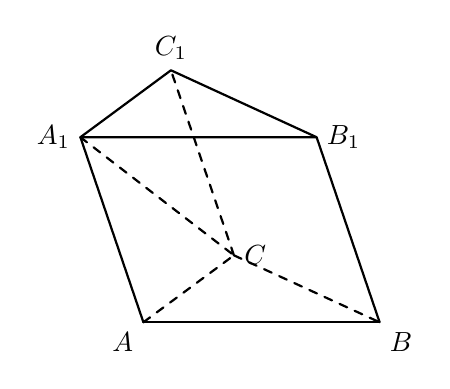
\begin{tikzpicture}[line cap=round,line join=round,thick]
  \coordinate (A) at (0,0);
  \coordinate (B) at (3,0);
  \coordinate (C) at (1.15,0.85);
  \coordinate (Aone) at (-0.8,2.35);
  \coordinate (Bone) at (2.2,2.35);
  \coordinate (Cone) at (0.35,3.2);

  % Hidden edges and the auxiliary segment shown dashed in the source.
  \draw[dashed] (A)--(C) (C)--(B) (C)--(Cone) (Aone)--(C);
  % Visible base, top, and lateral edges.
  \draw (A)--(B);
  \draw (Aone)--(Bone)--(Cone)--cycle;
  \draw (A)--(Aone) (B)--(Bone);

  \node[below left] at (A) {$A$};
  \node[below right] at (B) {$B$};
  \node[right] at (C) {$C$};
  \node[left] at (Aone) {$A_1$};
  \node[right] at (Bone) {$B_1$};
  \node[above] at (Cone) {$C_1$};
\end{tikzpicture}
